\documentclass[11pt]{article}
\usepackage{epsfig, latexsym, amsfonts}
\usepackage{graphicx}
\usepackage{enumerate}
\usepackage{enumitem}
%\usepackage{fancyhdr} % Required for custom headers
%\usepackage{lastpage} % Required to determine the last page for the footer
%\usepackage{extramarks} % Required for headers and footers
\usepackage[usenames,dvipsnames]{color} % Required for custom colors
\usepackage{color}
\usepackage{amsmath}
\usepackage{amsthm}
\usepackage{amssymb}
\usepackage{verbatim}
\usepackage[colorlinks=true, linkcolor = burgundy]{hyperref}
\usepackage{natbib}
%\usepackage{url}

\definecolor{burgundy}{rgb}{0.5, 0.0, 0.13}

\setlength\parindent{0pt}

% Margins
\topmargin=-0.6in
\evensidemargin=0in
\oddsidemargin=0in
\textwidth=6.5in
\textheight=9.0in
\headsep=0.25in

\linespread{1.1} % Line spacing

\setlength\parindent{0pt} % Removes all indentation from paragraphs

\newcommand{\beq}{\begin{equation}}
\newcommand{\eeq}{\end{equation}}
\newcommand{\bi}{\begin{itemize}}
\newcommand{\ei}{\end{itemize}}
\newcommand{\se}{\sigma_e}
\renewcommand{\sp}{\sigma_p}
\newcommand{\st}{\sigma_\theta}
\newcommand{\ai}{a_{i}}
\newcommand{\abar}{\bar{a}}
\newcommand{\pbar}{\bar{a}}
\newcommand{\shat}{\hat{\sigma}^2}
\newcommand{\hmu}{\hat{\mu}}
\newcommand{\mhat}{\hat{\mu}}
\newcommand{\svec}{\mathbf{s}}
\newcommand{\avec}{\mathbf{a}}
\newcommand{\bvec}{\mathbf{b}}
\newcommand{\hvec}{\mathbf{h}}
\newcommand{\calD}{\ensuremath{\mathcal{D}}}
\newcommand{\x}{\ensuremath{\mathbf{x}}}
\newcommand{\p}{\ensuremath{\mathbf{p}}}
\newcommand{\R}{\ensuremath{\mathbb{R}}}
\newcommand{\Z}{\ensuremath{\mathbb{Z}}}
\newcommand{\E}{\ensuremath{\mathbb{E}}}
\newcommand{\Et}{\ensuremath{\mathbb{E}_t}}
\newcommand{\Ett}{\ensuremath{\mathbb{E}_{t+1}}}
\newcommand{\cov}{\ensuremath{\mathbf{CoV}}}
\newcommand{\C}{\ensuremath{\mathbb{C}}}
\newcommand{\La}{\ensuremath{\mathcal{L}}}  %Lagrangian
\newcommand{\var}{\ensuremath{\mathbf{Var}}}  %Lagrangian
\newcommand{\B}{\ensuremath{\mathcal{B}}}    %topological basis
\newcommand{\Ps}{\ensuremath{\mathcal{P}}}  %power set
\newcommand{\Sp}{\ensuremath{\mathcal{S}}}  %power set
\newcommand{\I}{\ensuremath{\mathcal{I}}}  %power set
\newcommand{\pa}{\ensuremath{\mathbf{\alpha}}}
\newcommand{\pb}{\ensuremath{\mathbf{\beta}}}

\newcommand{\info}{\mathcal{I}_i}
\newcommand{\infoset}{\mathcal{I}_i}
\newcommand{\onevec}{\mathbf{1}}

\title{First Time Home Buyers Age Distribution: A Simple Model}

\date{ }

\renewcommand{\cite}{\citep}
\newcommand{\citeasnoun}{\citet}
\newcommand{\harvardcite}{\citet}
\theoremstyle{definition} %plain italicizes stuff
\newtheorem{problem}{Problem}
\newtheorem{assumption}{Assumption}
\newtheorem{solution}{Solution}
\newtheorem{axiom}{Axiom}
\newtheorem{example}{Example}
\newtheorem{definition}{Definition}
\newtheorem{result}{Result}
\newtheorem{prop}{Proposition}
\newtheorem{cor}{Corollary}
\newtheorem*{theorem}{Theorem}
\DeclareMathOperator*{\argmin}{arg\,min}
\DeclareMathOperator*{\argmax}{arg\,max}

\begin{document}

\maketitle


\section{Continuous Time Model}
\subsection{Environment}
The economy is populated by households at different ages. We assume that households start working at the age of 20 and there wealth evolves according to the following diffusion process
\[
dw_t^i = \mu dt + \sigma dB_t^i ~,
\]
where $\exp(w_t^i)$ is the wealth of household $i$ at age $20+t$. $B_t^i$ is a standard Brownian motion (which is independent across $i$'s). For simplicity, we assume that the household's initial wealth is equal to 1 so that $w_0 = 0$.\\
Denote the price of housing to be $p_H$. We assume this price is constant over time. Let $\theta$ be the fraction that must be paid when purchasing a house. Finally, we assume that whenever a household has enough wealth to pay the down payment and purchase a house it does so. Thus, the time in which a household purchases a house is given by
\[
\tau^i = \inf_s \left\{s: w^i_s\geq \ln \left(\theta p_H\right) \right\}
\]

We now turn to characterize the distribution $\tau^i$'s in the economy as a function of the fundamental exogenous parameters ($p_H,~ \theta,~ \mu,$ and $\sigma$).
\subsection{First Time Home Buyers Age Distribution}
In this section we characterize the distribution of $\tau^i$. Notice that $\tau^i$ is simply a stopping time so that we can use known mathematical results regarding the distribution of stopping times.
\begin{prop}
The density of $\tau^i$ is given by
\[
f_\tau (t) = \frac{\ln (\theta p_H)}{\sigma \sqrt{2\pi t^3}} \exp \left\{ -\frac{(\ln (\theta p_H) - \mu t)^2}{2\sigma^2 t} \right\}
\]
\end{prop}
\begin{proof}
A trivial modification of the proof provided here: \url{http://math.stackexchange.com/questions/1053294/density-of-first-hitting-time-of-brownian-motion-with-drift}
\end{proof}
\textbf{Calibration.} Let $p_H = 10e$ and let $\theta = 0.1$. We shall calibrate $\mu$ to $1/12$ so that without the diffusion term it would take a household 12 years to purchase a house (such household would be 32 years old). Finally, we let $\sigma = 0.15$. Figure \ref{age_dist} displays the distribution of first time home buyers age given this calibration. The mode is at age 28, while the expected age of purchasing a house is at age 32.


\begin{figure}[h!]
\centering
\caption{Age Distribution} \label{age_dist}
\vspace{3mm}
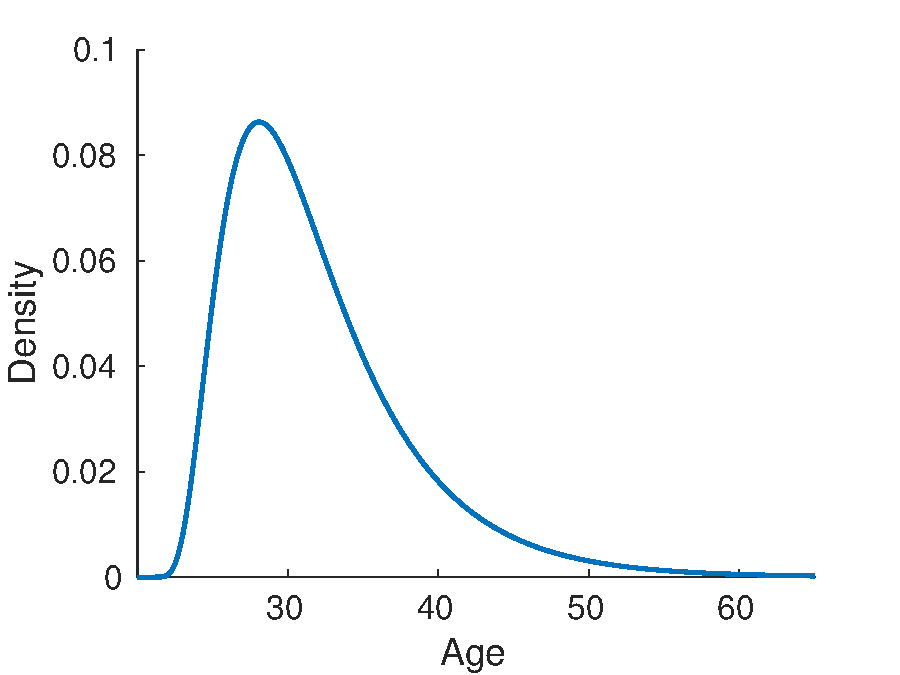
\includegraphics[scale=0.6]{fthb_age_dist.pdf}
\end{figure}
\subsection{Comparative Statics}
The 4 graphs in Figure \ref{CS} display the distribution varying the 4 exogenous parameters each at a time.

\begin{figure}[h!]
\centering
\caption{Age Distribution - Comparative Statics} \label{CS}
\vspace{2mm}
\begin{tabular}{c c c}
$p_H = 15e$ && $\theta = 0.15$ \\
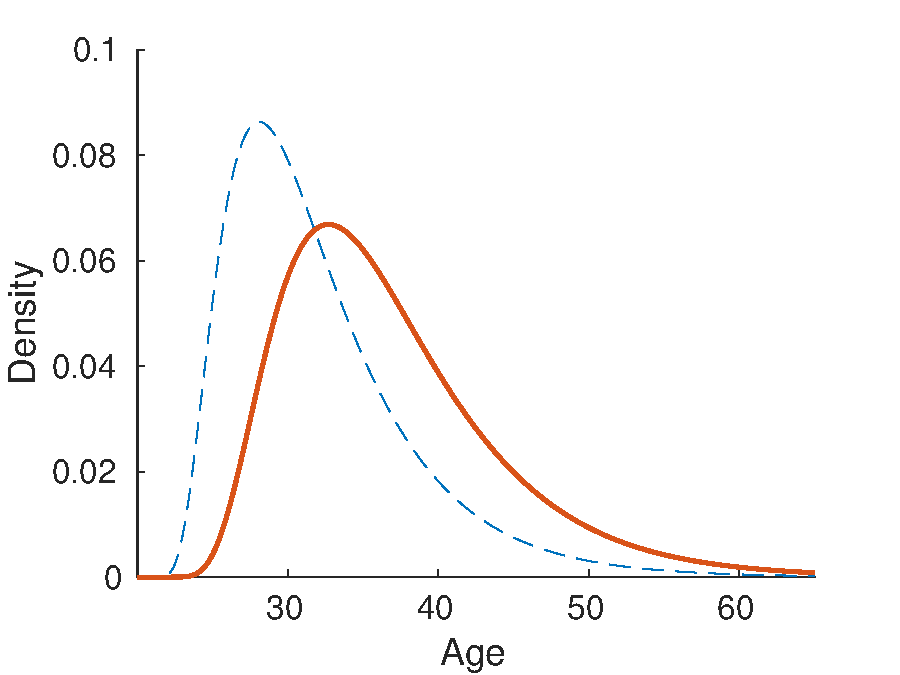
\includegraphics[scale=0.4]{CS1.pdf} && 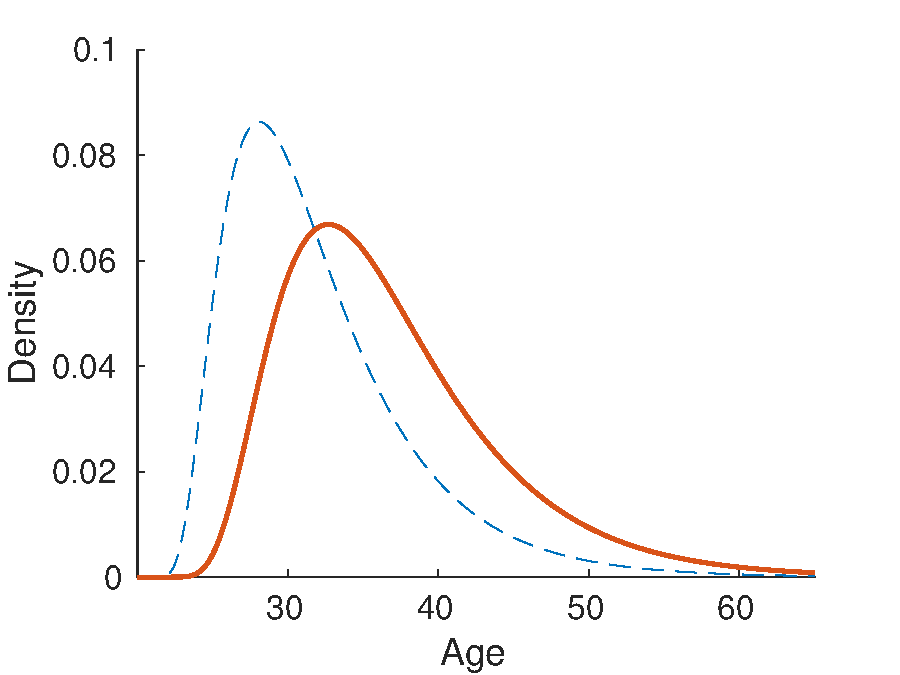
\includegraphics[scale=0.4]{CS2.pdf} \\ \\
$\mu = 1/15$ && $\sigma = 0.2$\\
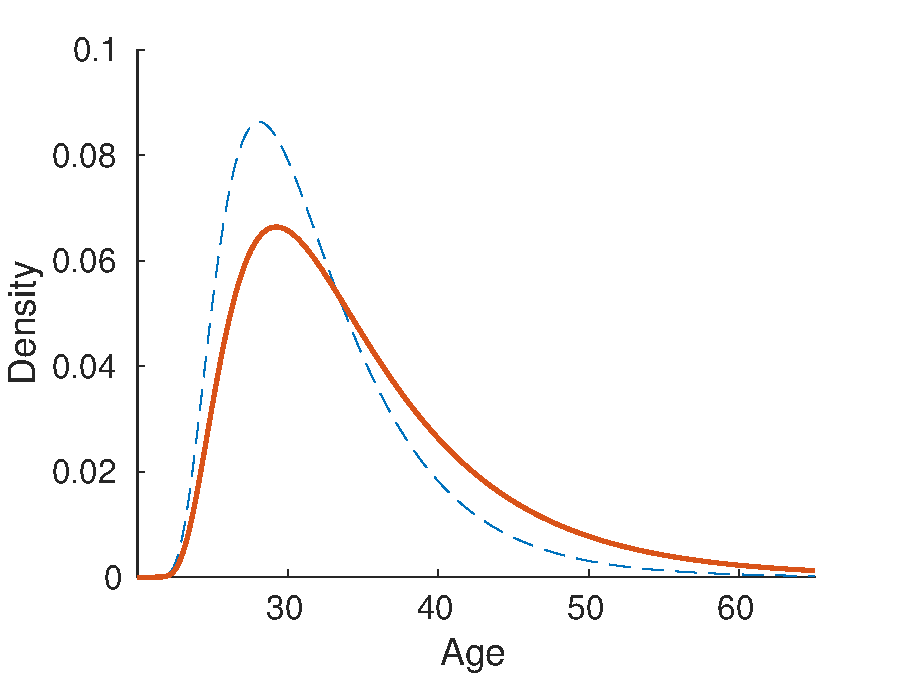
\includegraphics[scale=0.4]{CS3.pdf} && 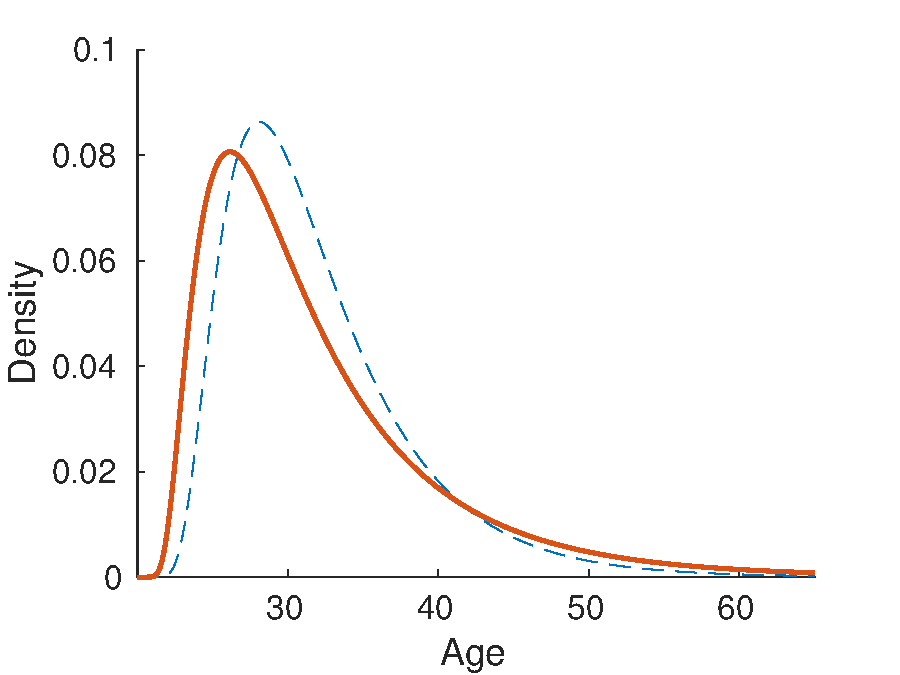
\includegraphics[scale=0.4]{CS4.pdf} 
\end{tabular}

\end{figure}
\end{document}
